\begin{center}
    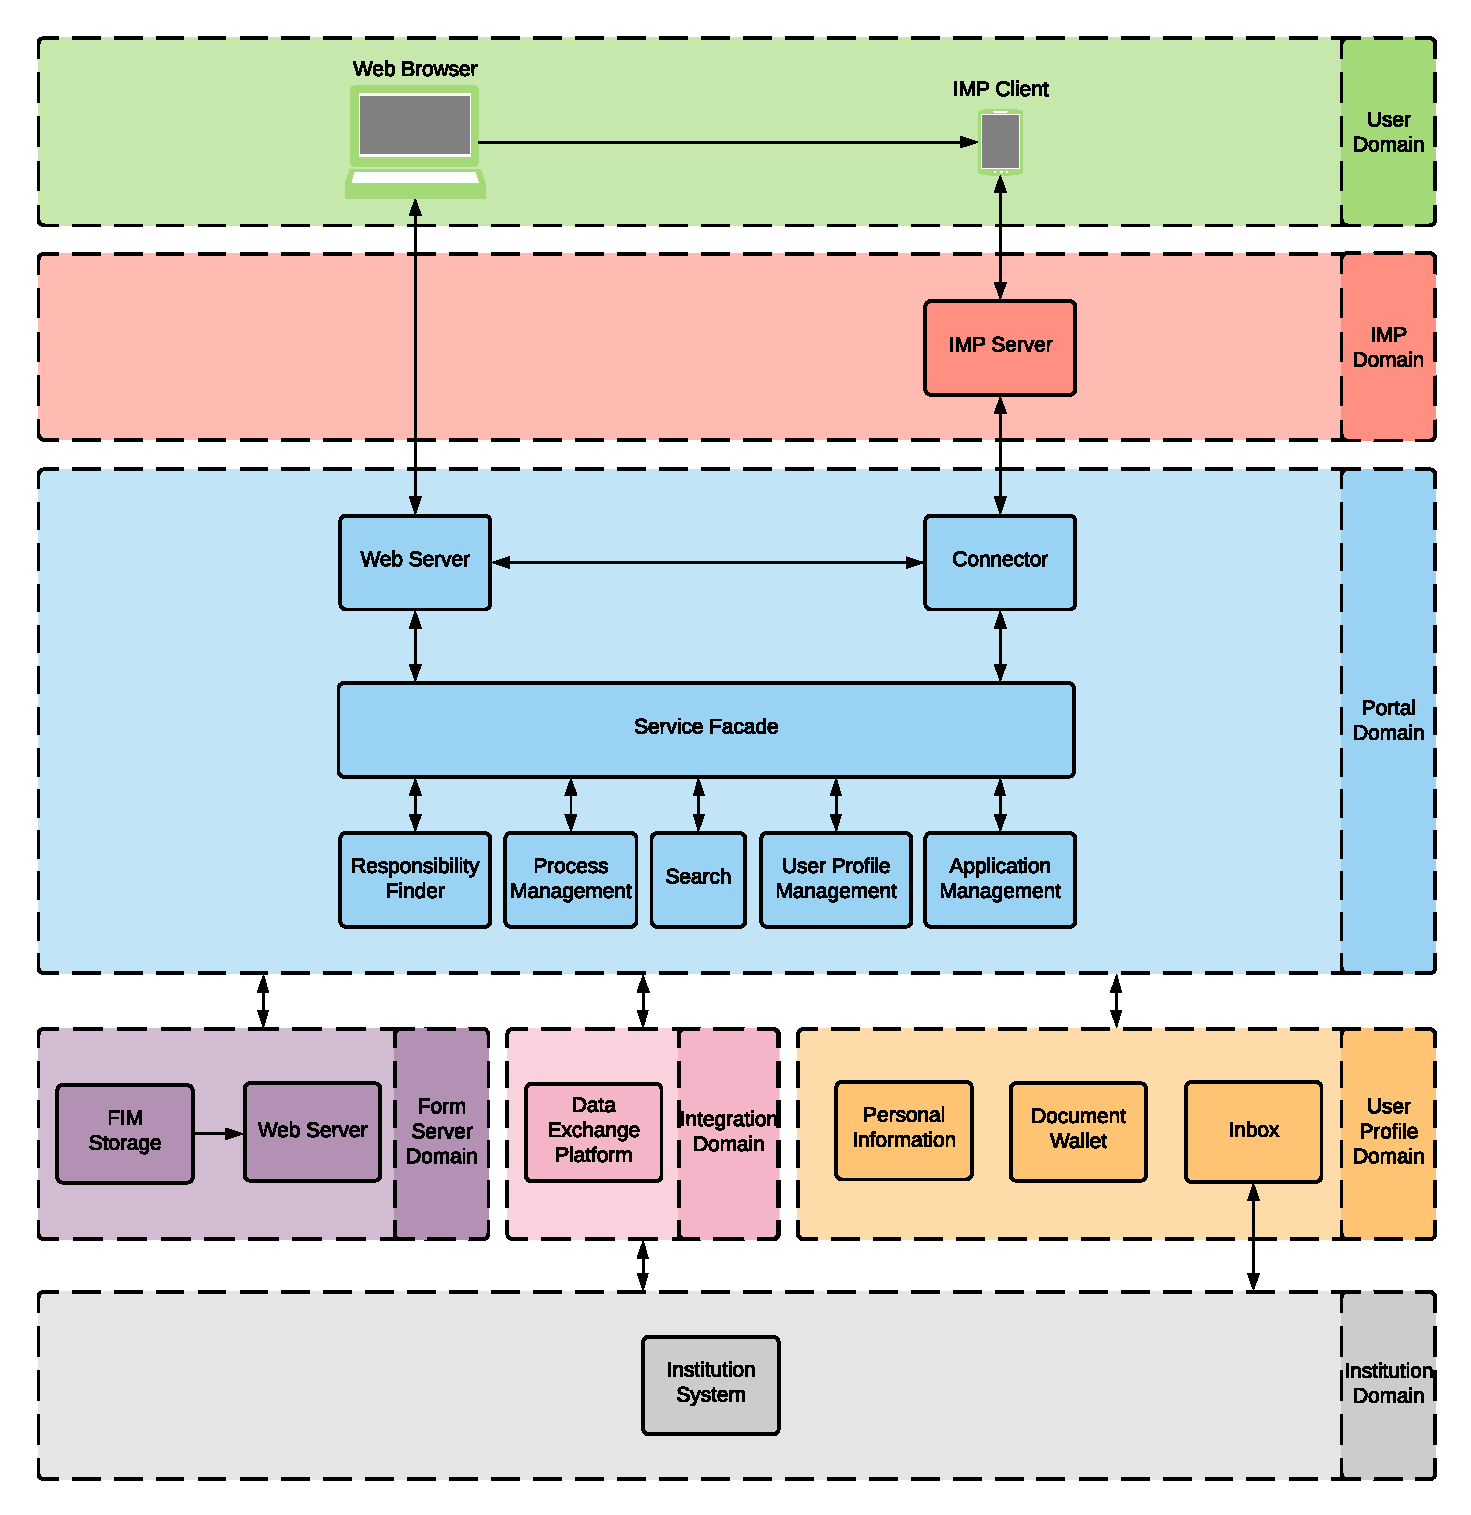
\includegraphics[scale=0.6]{Diagrams/Integration Architecture 1/Overview.pdf}
\end{center}

For the existing system architecture to access the IMP system, an IMP connector is added to the portal domain. The connector communicates with an IMP client trough the IMP server located in the IMP domain.

\begin{center}
    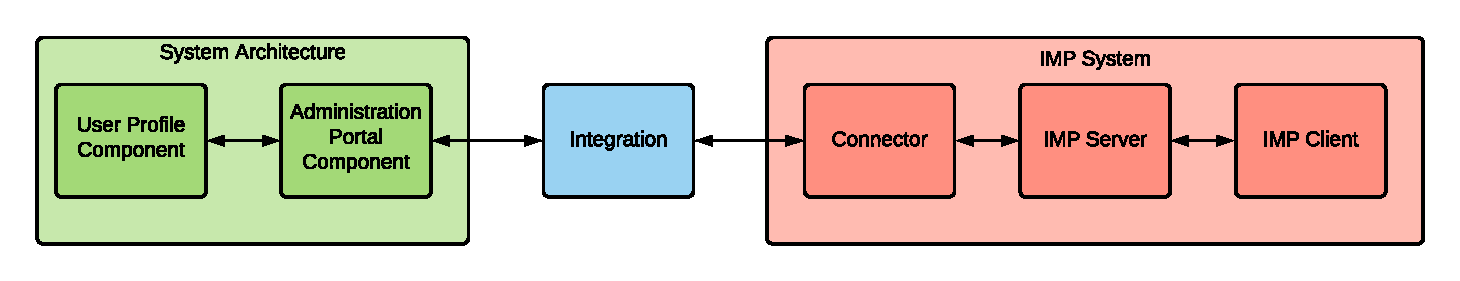
\includegraphics[scale=0.6]{Diagrams/Integration Architecture 1/Technological Integration/2. System Overview.pdf}
\end{center}

System architecture of the SP and IMP system consist of multiple components. The administration portal component of the system architecture  will interact with the integration system. The administration portal contains a web server and a service facade. The service facade enables the administration portal amongst other things to access the user profile component. On the side of the IMP system, the connector will interact with the integration system.

\begin{center}
    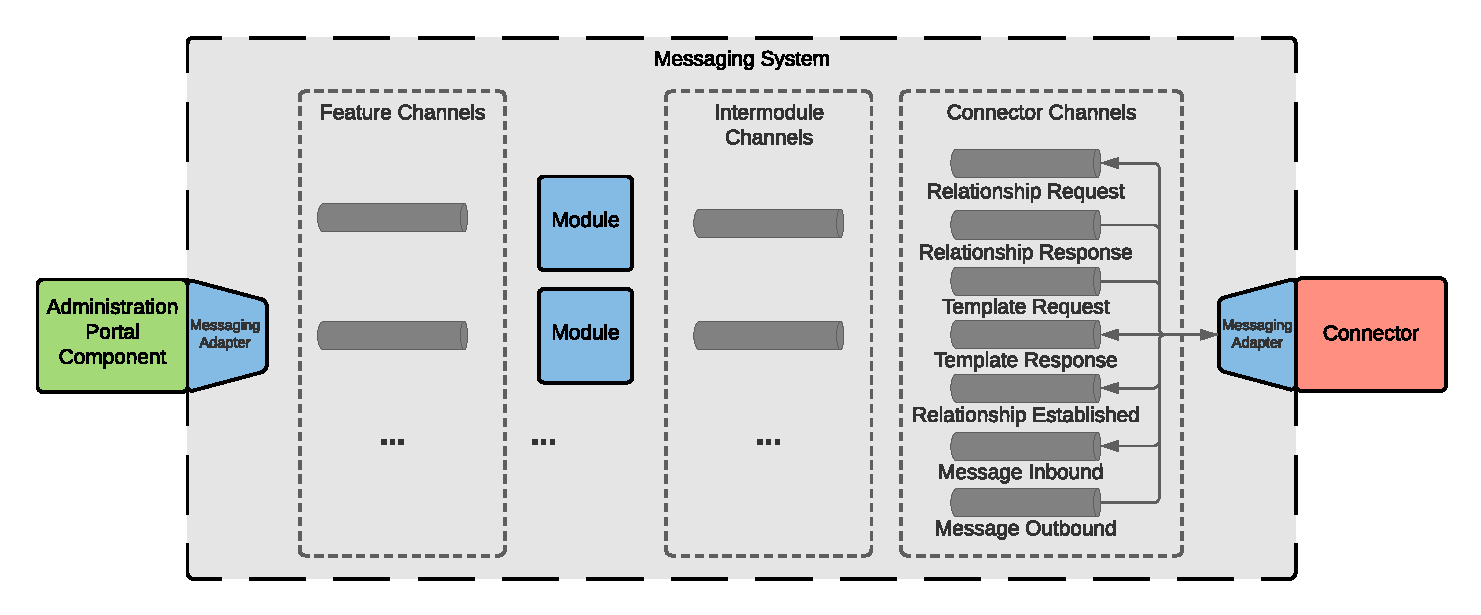
\includegraphics[scale=0.6]{Diagrams/Integration Architecture 1/Technological Integration/4. Messaging Overview.pdf}
\end{center}

The integration is constructed as a messaging system. The messaging system consists of modules which exchange messages with connector and administration portal. As administration portal and connector are not able to send, receive or understand messages, a messaging adapter is attached to both systems. A messaging adapter is software which provides an API to the system hiding the operation of the messaging system. Depending on the system the messaging adapter should be attached to, different integration methods can be used. In most cases however, manual modification of the programming of the system is necessary to utilize the API of the adapter.

The integration system consists of messaging modules, each of them solving a different integration task. The modular approach enables the integration system to be easily expandable by new features trough new modules. Assigning integration tasks to modules also improves maintenance. System administrators can update a feature by modifying and expanding the corresponding module.
Modules can be designed to be reusable by other components which reduces the development time for new features and the size of the integration system. If the modules supports it, the performance of the integration system can be dynamically scaled by adding more module instances.

Modules have the purpose of solving integration tasks by providing access to features presented in section 5.1 while hiding the complexity of the operation of the IMP system. They exchange messages through three types of publish-subscribe channels. Between administration portal and modules, feature channels are used. On these channels, messages strongly related to the operation of the system architecture of the service provider are exchanged. This are for example messages for requesting services like the transmission of a mail.

Between modules and connector, connector channels are used. These are a predetermined and limited set of channels which are used by the messaging adapter to map the functionalities of the connector to the messaging system. Messages exchanged on these channels are strongly related to the operation of the IMP system. This are for example requests and replies for relationships and templates.

Between modules, intermodule channels are used to exchange messages. Modules can exchange messages in order to access distributed functionalities of other modules.

\begin{center}
    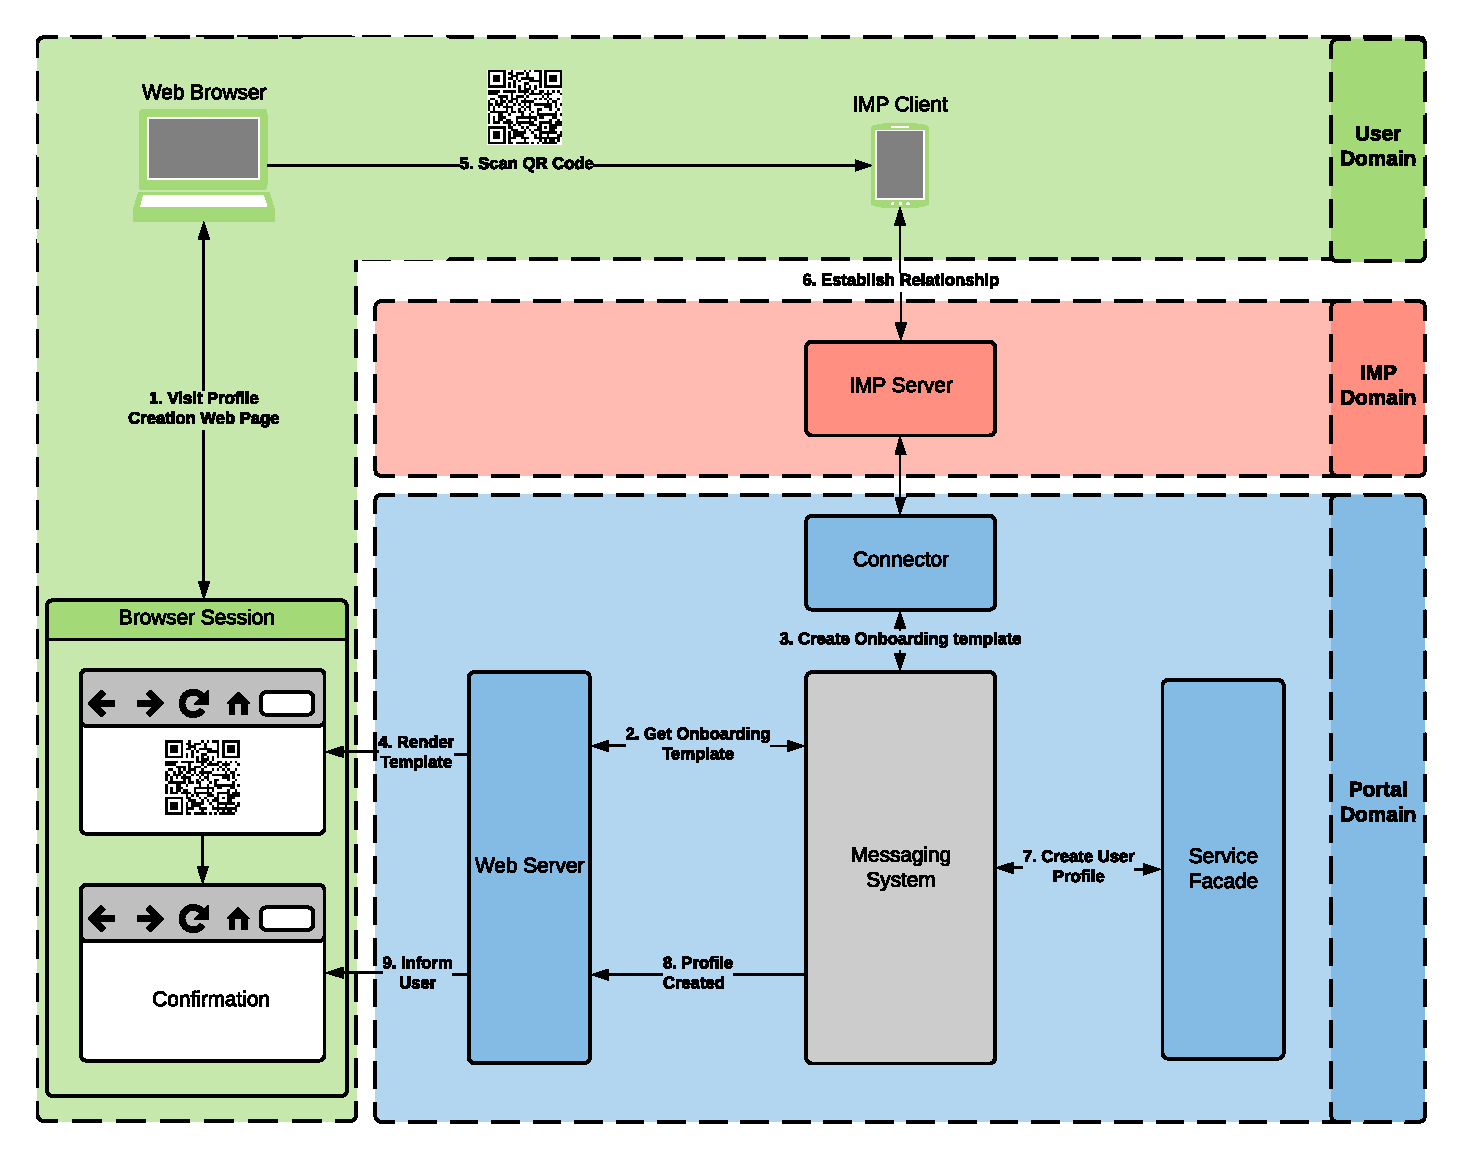
\includegraphics[scale=0.6]{Diagrams/Integration Architecture 1/Technological Integration/5. Onboarding Overview.pdf}
\end{center}


As described in section 5.1, the user should be able to create a new user profile for the OZG system through an existing IMP identity.

On the existing website of the administration portal, where users can create a user profile, the relationship template for onboarding should be displayed. When the web server receives a GET request for the profile creation website, it issues a request to the messaging system for a new onboarding template. The messaging system interacts with the IMP connector to construct the template and send it back to the web server. The web server renders the template as a QR code. The QR code is displayed on the device of the user who can use the IMP client to scan it and initiate a relationship request. The messaging system interacts with the connector to establish the relationship and eventually issues the service facade to create a new user profile based on the attributes shared as part of the IMP relationship. After successful creation of the user profile, the messaging system stores the relationship ID and the user profile ID in a database. In the future, each request containing either a user profile ID or relationship ID can be mapped to the correct OZG and IMP identities. The messaging system notifies the web server of the successful creation of the user profile and the web server displays a corresponding notification to the user.

\begin{center}
    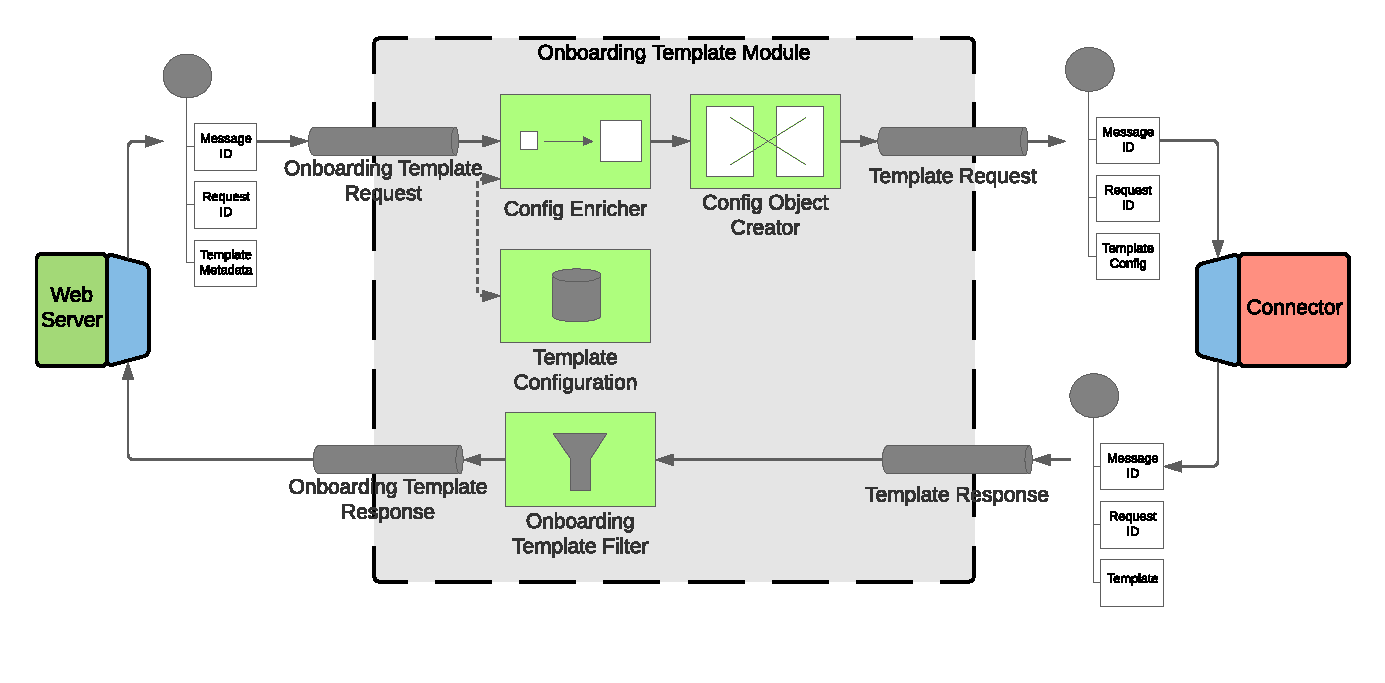
\includegraphics[scale=0.6]{Diagrams/Integration Architecture 1/Technological Integration/6. Onboarding Template Module.pdf}
\end{center}

To present an onboarding relationship template to the user, the web server first has to retrieve it from the integration system. For this purpose, an "Onboarding Template Module" is added to the messaging system. Using the API of a messaging adapter provided in addition to the module, the web server can request the creation of new onboarding templates. Optionally, the web server can pass additional attributes which should be stored in the metadata section of the template. In this case, the web server will want to notify the user about the successful creation of his user profile. The web server therefore adds the users current session ID as metadata to the template.

The messaging adapter is aware of the existence of two channels: the "Onboarding Template Request" channel, where it publishes its requests and the "Onboarding Template Response" channel, where it listens for responses. In order for the adapter to correlate request and reply messages, it creates a message which besides the Template Metadata contains a request ID. This ID is expected to be included in the response message. The message ID is a unique identifier and is part of every message. The module consumes messages from the "Onboarding Template Request" channel and adds an configuration object stored at a database. This configuration contains information on how relationship templates of type onboarding are supposed to look like. It specifies the title of the template, which attributes will be requested from the user, the reason why the attributes are requested and more. If the content of relationship templates should be changed in the future, depending on the severity of the changes, either a new template module can be created or the configuration stored in the database can be edited.

Purpose of the relationship template is to eventually create a new user profile based on the attributes shared by the IMP identity. Therefore, all attributes which are required to create a user profile have to be requested by the template. As the data model of the OZG systems and IMP systems are different, message translators will have to be used to translate between them. Therefore, most modules will contain a component called "Attribute Mapping" which is responsible for translating the attribute definitions of the IMP system to attribute definitions of the OZG system and vice versa. In this model however, no message translator is required, as the configuration of the template can be defined to use the IMP data model.

A message translator combines template metadata and configuration to a configuration object, the connector understands and publishes it on the "Template Request" channel.

The messaging adapter of the connector issues the appropriate REST request to the connector and publishes the resulting template along with the request ID on the "Template Response Channel". As this channel can contain responses to requests from any amount of modules concerning different template types, the "Onboarding Template Module" filters all incoming messages which contain templates of the type "onboarding" and publishes them on the "Onboarding Template Response" channel.

The messaging adapter returns the template to the web server, which based on the session ID in the template metadata can display the template as QR code to the user.


\begin{center}
    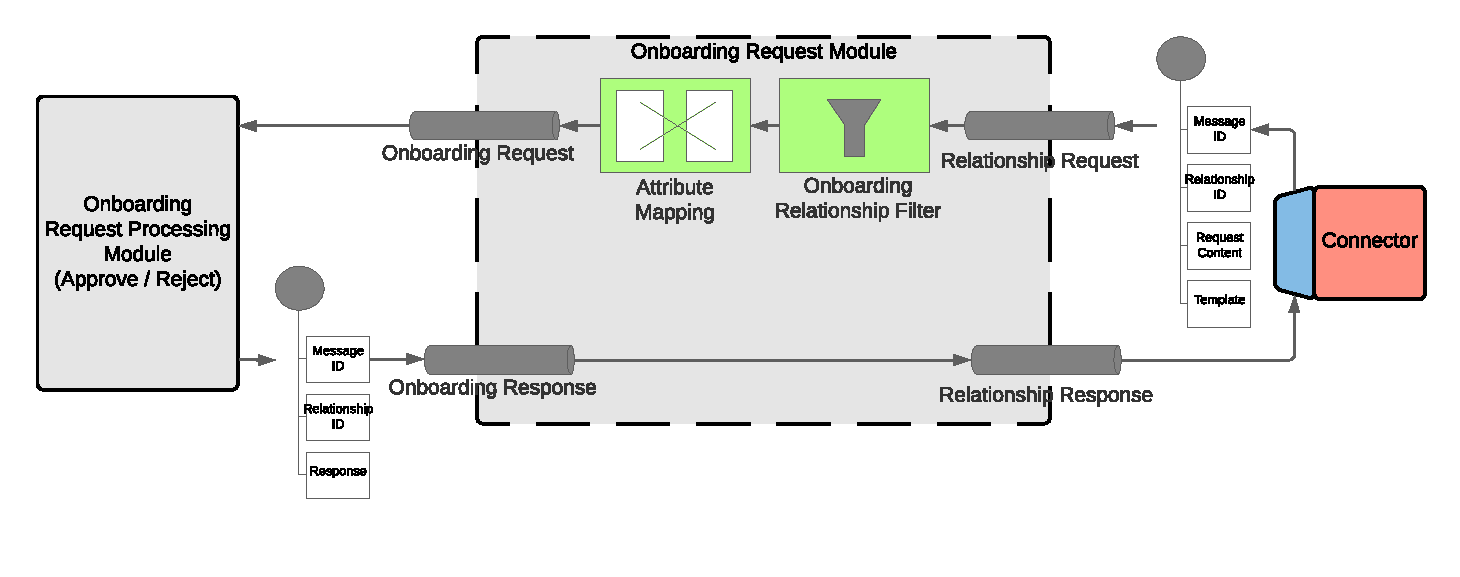
\includegraphics[scale=0.6]{Diagrams/Integration Architecture 1/Technological Integration/7. Onboarding Request Module.pdf}
\end{center}

Eventually, the user scans the QR code, fills in the attributes and submits a relationship request. The request is received by the connector, forwarded to the messaging adapter and published on the "Relationship Request" channel. The message contains a relationship ID created by the IMP server to uniquely identify the request and the resulting relationship. It also contains the request content with attributes shared by the user and the template the request originated from. Messages on the "Relationship Request" channel are consumed by the "Onboarding Request Module". A message filter only lets messages trough which contain templates of type onboarding. A message translator translates attributes shared by the user from the IMP data model to the OZG data model and publishes the message on the "Onboarding Request" channel.

Based on the attributes the user shares, the OZG system has to decide if the relationship should be established or not. As this process heavily depends on the use case of the relationship and on the service provider, the messaging system expects the SP to add a module called "Onboarding Request Processing Module" which consumes the request and responds with either approve or reject on the "Onboarding Response" channel. To correlate the response to the request, the message also has to contain the relationship ID. The "Onboarding Request Module" forwards the response to the "Relationship Response" channel, where the connector will further interact with the IMP system to either establish or cancel the relationship. In between a message translator can, if required, translate the format of the response attribute so that the connector understands it.

\begin{center}
    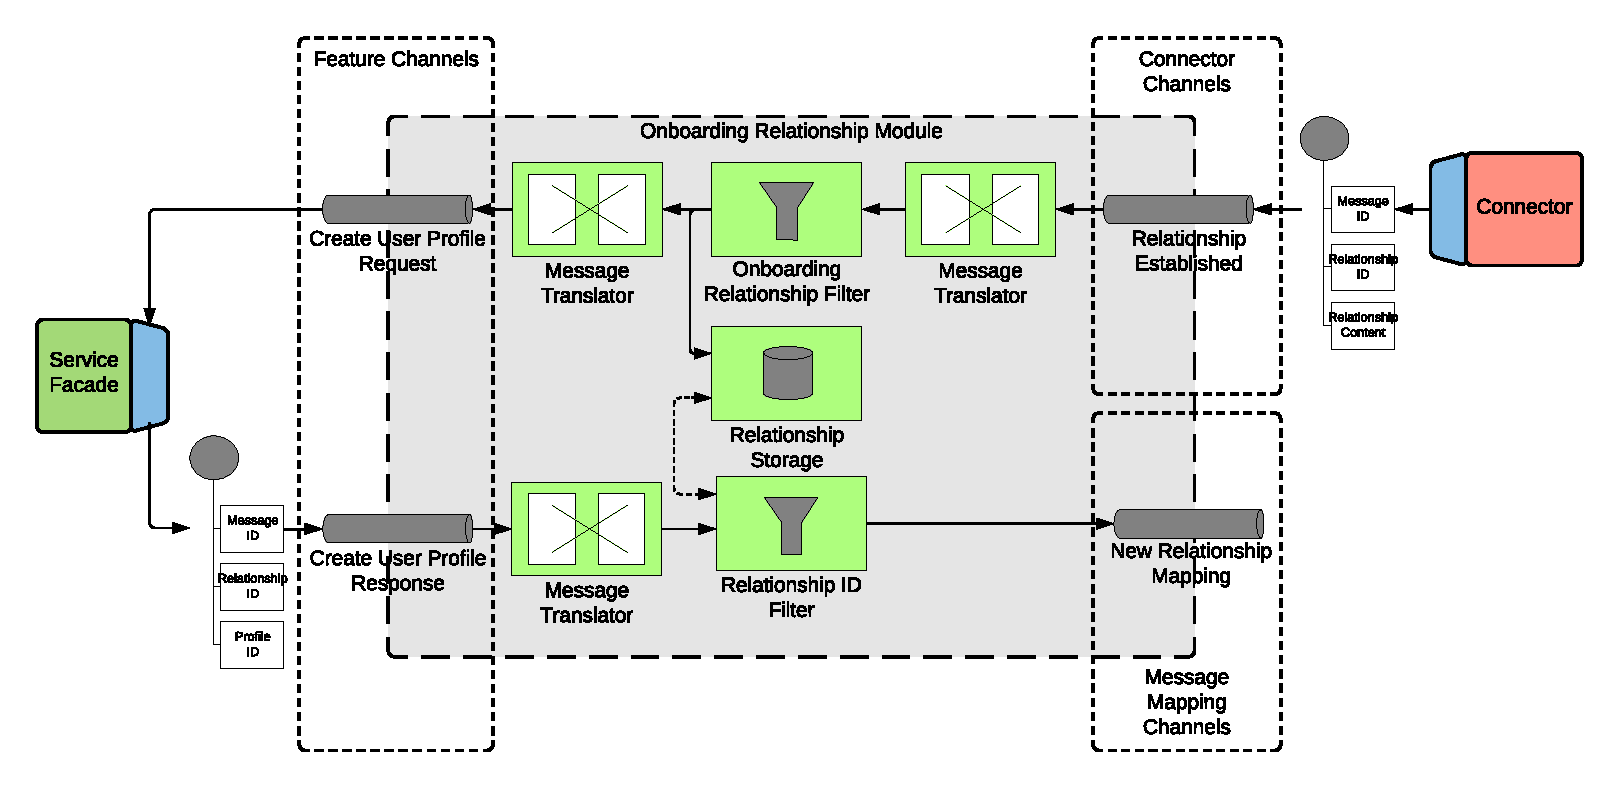
\includegraphics[scale=0.6]{Diagrams/Integration Architecture 1/Technological Integration/8. Onboarding Relationship Module.pdf}
\end{center}

If the user did not retract his relationship request before the OZG system accepted it, the relationship is established and the connector receives a corresponding notification which the messaging adapter publishes on the "Relationship Established" channel. The message contains the ID of the established relationship along with all attributes shared by the user. The "Onboarding Relationship" module consumes messages from the channel and is responsible for maintaining the state of onboarding relationships. In this case, the module only processes the establishing of relationships, it could however be expanded to also process terminations of relationships.

The module processes an established relationship by initiating the creation of a new user profile. First, a message filter lets trough only messages of the onboarding type. Afterwards, each message is stored in a "Relationship Storage" database and published on the "Create User Profile Request" channel. However, before publishing the message, attributes are again mapped form the IMP data model to the OZG data model.

To create a user profile, a messaging adapter attached to the service facade of the administration portal consumes messages from the "Create User Profile Request" channel and issues the corresponding requests to the service facade for creating a new user profile based on the attributes stored in the relationship content. After successful creation of the user profile, the messaging adapter publishes a response message on the "Create User Profile Response" channel which contains the relationship ID and the newly created Profile ID.

As responses to requests from other modules might be published on this channel, the "Onboarding Relationship" module filters all messages which do not contain a relationship ID stored in the "Relationship Storage". The rest of the messages is stored in a "Profile ID / Relationship ID Mapping" database. 

This database is used trough intermodule communication to map profile IDs to relationship IDs and vice versa. Modules can publish messages on the "Identity Mapping Request" channel either containing a relationship ID or profile ID attribute and receive the message containing both profile ID and relationship ID on the "Identity Mapping Response" channel. Using messaging for this form of database access enables modules to stay unaware of the complexities of the underlying data storage mechanisms. An alternative would be for modules to use the database as a shared database.

\begin{center}
    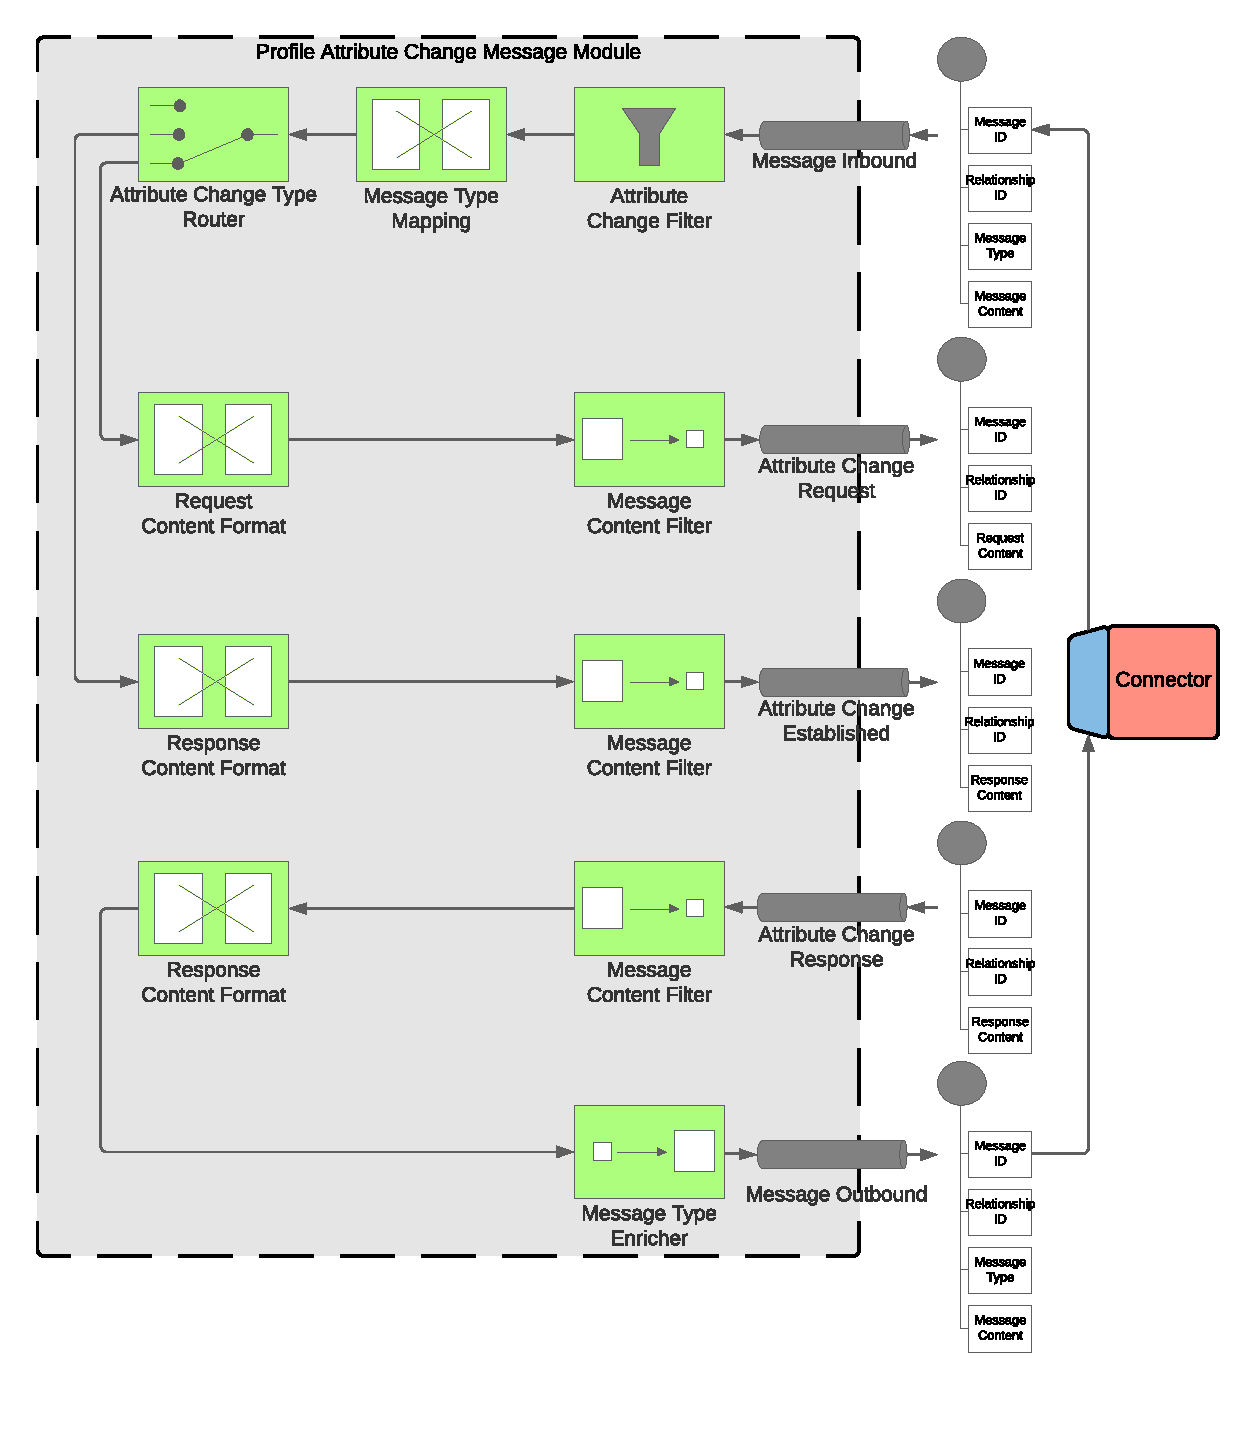
\includegraphics[scale=0.6]{Diagrams/Integration Architecture 1/Technological Integration/9. Attribute Change Message Module.pdf}
\end{center}

For the messaging system to process messages being exchanged as part of relationships, message modules can be added. Their purpose is to map messages of certain types on the "Message Inbound" channel to individual message type channels so that modules can process them. They also map messages of the individual message type channels to the "Message Outbound" channel to so that the connector can submit them.

In this case, an "Attribute Change Message Module" is included, which processes messages related to the attribute change process of onboarding relationships. The connector receives a message corresponding to a relationship ID which the messaging adapter publishes on the "Message Inbound" channel. The message contains the ID of the relationship it was exchanged trough, an identification of the message type and the content of the message. Message type and content can be freely specified by the IMP client, however only certain message types are understood by message modules and only certain message contents can be processed by the integration system. The integration architecture will therefore have to adhere to the standard the IMP client specifies and adapt to possible future changes.

The "Attribute Change Message Module" consumes messages on the "Message Inbound" channel and filters all messages with types not related to attribute change. A message translator translates incoming message types to types the integration architecture can processes. This can be necessary, if for example the IMP client changes definitions of message types. A message router routes the messages to different channels depending on their type. In this case, two types of incoming messages can be processed on the "Attribute Change Request" channel and on the "Attribute Change Established" channel. To expand the list of message types the integration architecture can process, corresponding channel can be added.

Before publishing messages on the channels, a message translator translates the message content to a format, the integration architecture understands. This might be possible if in the future, the IMP client changes the format. A content filter removes unnecessary content from the message such as the message type, as modules will be able to infer it from the channel a message is published on.

The module is also able to process outbound messages originating from one of the modules. In this case, messages can arrive on the "Attribute Change Response" channel. A content filter removes unnecessary attributes attached to the message. In order to adapt to changes in the response format the IMP client understands, a message translator is attached. For the IMP client to understand the message, the implicit message type of the channel has to be added aThe module s an attribute. The resulting message is then published on the "Message Outbound" channel, where the messaging adapter instructs the connector to submit it.

\begin{center}
    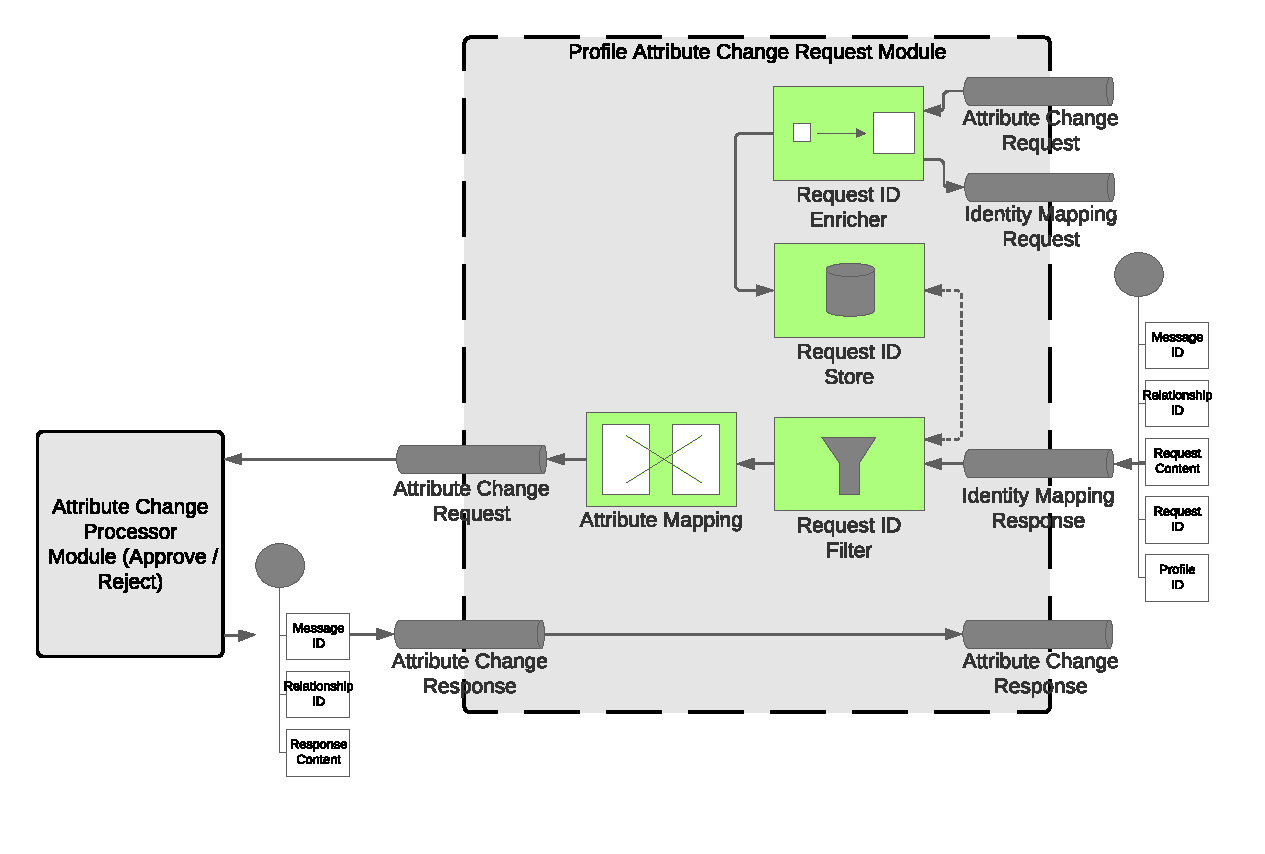
\includegraphics[scale=0.6]{Diagrams/Integration Architecture 1/Technological Integration/10. Attribute Change Request Module.pdf}
\end{center}

To process incoming attribute change requests for profiles, a "Profile Attribute Change Request" module is included which consumes messages from the "Attribute Change Request" channel. To retrieve the user profile ID connected to the relationship ID, an incoming message is forwarded to the "Identity Mapping Request" channel. To eventually correlate the reply to the request, a content enricher adds a request ID to the message and stores the ID in a "Request ID Store".

Replies on the "Identity Mapping Response" channel which do not contain a request ID stored in the "Request ID Store" are filtered. The other messages are consumed by a message translator which, such as in previous modules, maps attributes shared as part of the attribute change request from the IMP data model to the OZG data model an publishes the message on the "Attribute Change Request" channel.

Similar to the "Onboarding Request Module", the decision whether to approve or reject an attribute change is specific to the service provider. Therefore, the SP is expected to include an "Attribute Change Processor" module, which based on the attribute change request, the relationship ID and the profile ID decides to approve or reject. The response is published to the "Attribute Change Response" channel and besides the response content contains the relationship ID.

The "Profile Attribute Change Request" module forwards the message to the "Attribute Change Response" channel, where the message module will further process it for delivery to the connector.

\begin{center}
    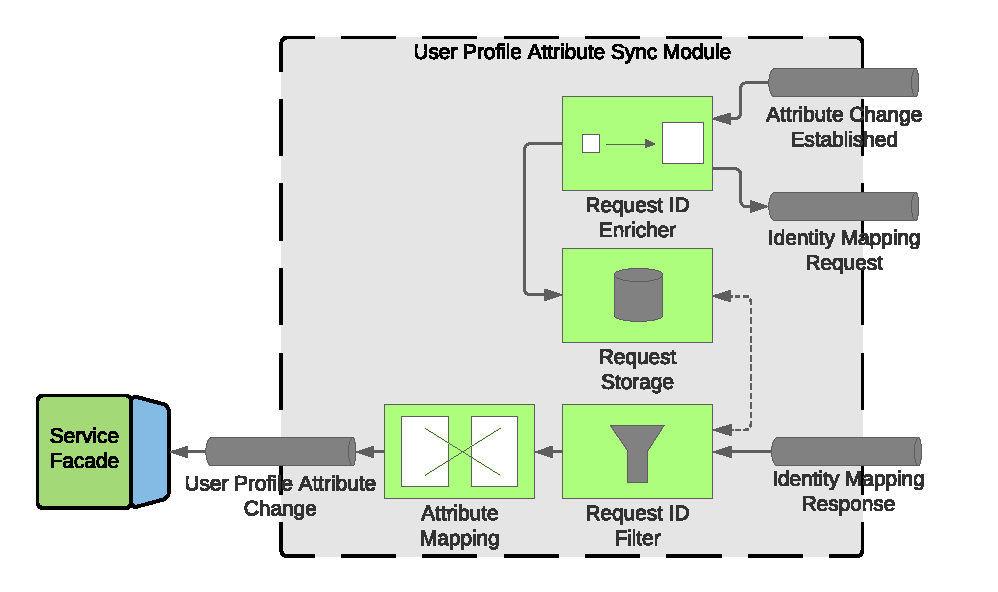
\includegraphics[scale=0.6]{Diagrams/Integration Architecture 1/Technological Integration/11. User Profile Attribute Sync Module.pdf}
\end{center}

If the user did not cancel the attribute change request before the OZG system accepted, the attribute change is established. The connector is notified trough a message, which eventually the "Profile Attribute Change Message" module described earlier will process and publish on the "Attribute Change Established" channel.

The "User Profile Attribute Sync" module consumes messages from the "Attribute Change Established" channel and similar to the "Profile Attribute Change Request" module, retrieves the profile ID corresponding to the relationship ID. Before publishing the response on the "User Profile Attribute Change" channel, the attributes are again translated from the IMP data model to the OZG data model. A channel adapter connected to the service facade consumes the message and updates the specified attributes for the specified user profile. 

\begin{center}
    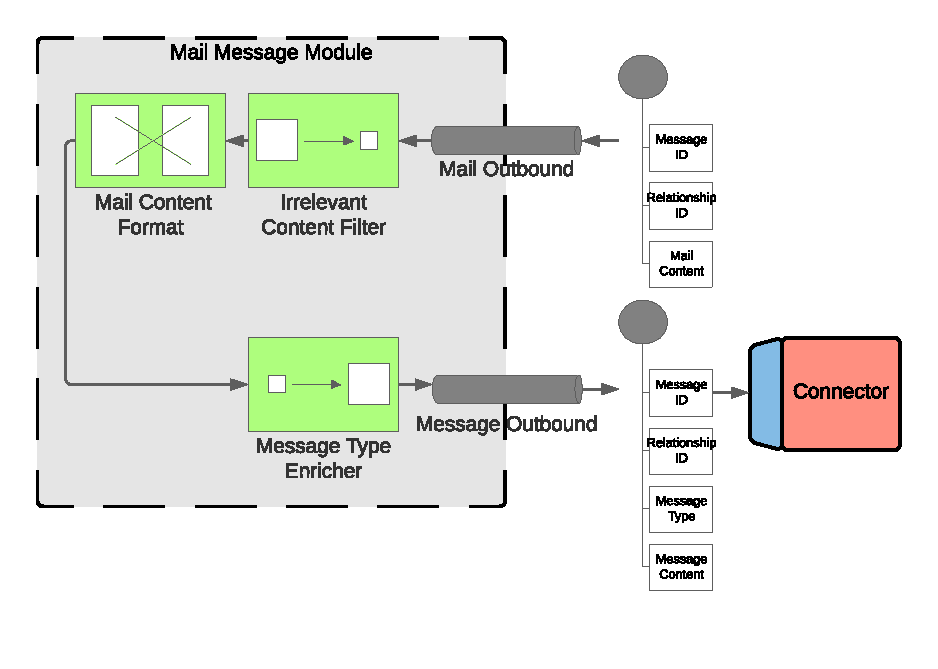
\includegraphics[scale=0.6]{Diagrams/Integration Architecture 1/Technological Integration/12. Mail Message Module.pdf}
\end{center}

In order for the user to receive messages sent to his user profile trough the IMP client, mail messages are processed by the integration architecture. Similar to the "Profile Attribute Change Message" module, a "Mail Message" module is included, which maps messages on the "Mail Outbound" channel to the "Message Outbound" channel.

In this module, incoming mails from the IMP client could also be processed, however this option is not included in the integration.

Trough a content filter, the module removes unimportant attributes from the message. A message translator is sued to translate the mail format of the user profile inbox to the format of the IMP client inbox. Eventually, a content enricher adds the implicit message type of the channel as attribute in order for the IMP client to understand it and publishes it on the "Message Outbound" channel. 

\begin{center}
    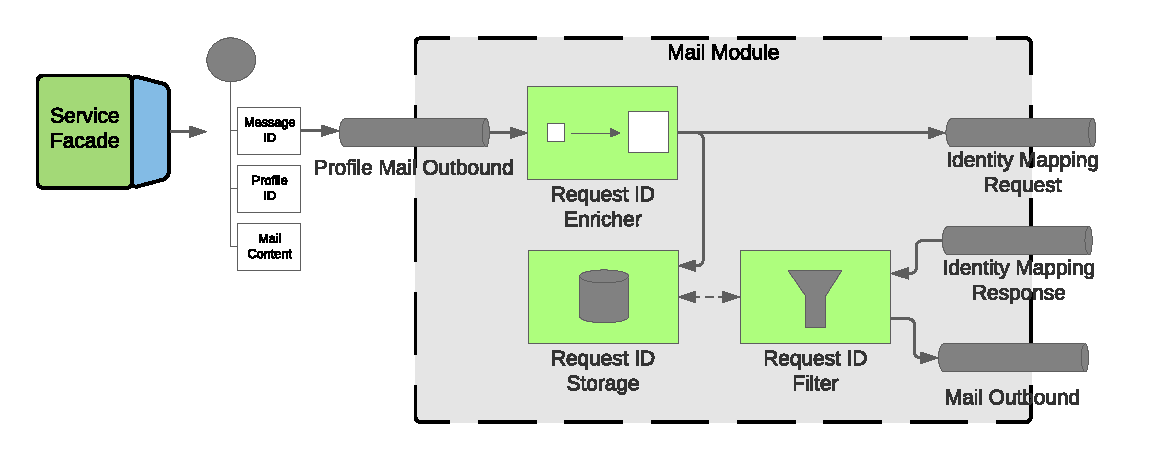
\includegraphics[scale=0.6]{Diagrams/Integration Architecture 1/Technological Integration/13. Mail Module.pdf}
\end{center}

An messaging adapter attached to the service facade is notified each time, a user profile connected to an IMP identity receives a mail and publishes a message on the "Profile Mail Outbound" channel. The message contains the ID of the profile which received the message and the content of the mail. A "Mail" module is included which consumes the messages from the "Profile Mail Outbound" channel, retrieves the corresponding relationship ID, similar to previous modules, and publishes them on the "Mail Outbound" channel. The messages on the "Mail Outbound" channel are processed by the "Mail Message" module described earlier.

\begin{center}
    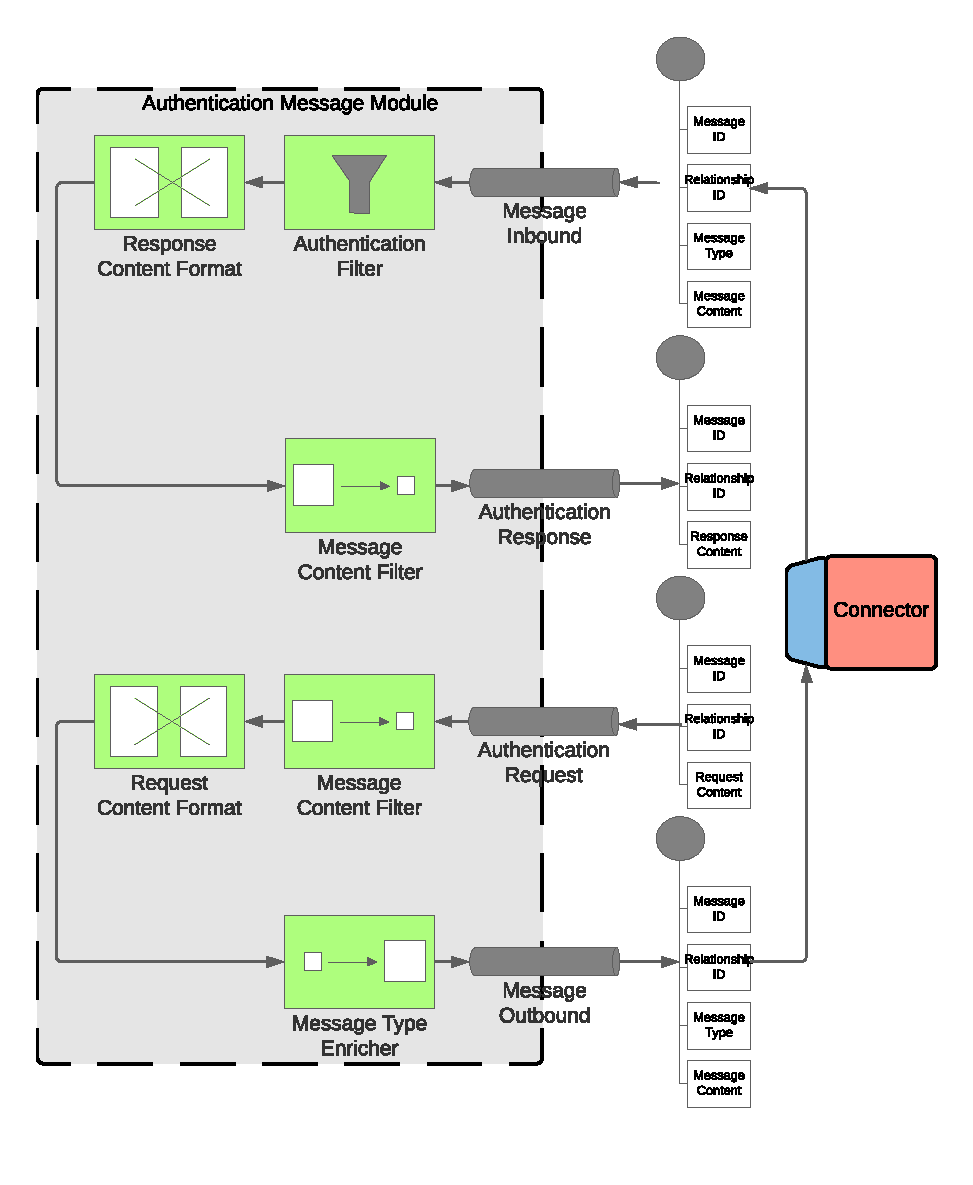
\includegraphics[scale=0.6]{Diagrams/Integration Architecture 1/Technological Integration/14. Authenticatin Message Module.pdf}
\end{center}

If the user creates a user profile using his IMP identity, it is possible to replace authentication using a password with authentication trough the IMP client. It is also possible to use the IMP client for two factor authentication.

In order to send and receive messages related to authentication, similar to previous message modules, a "Authentication Message" module is included which maps incoming messages on the "Message Inbound" channel to the "Authentication Response" channel and outgoing messages from the "Authentication Request" channel to the "Message Outbound" channel.

\begin{center}
    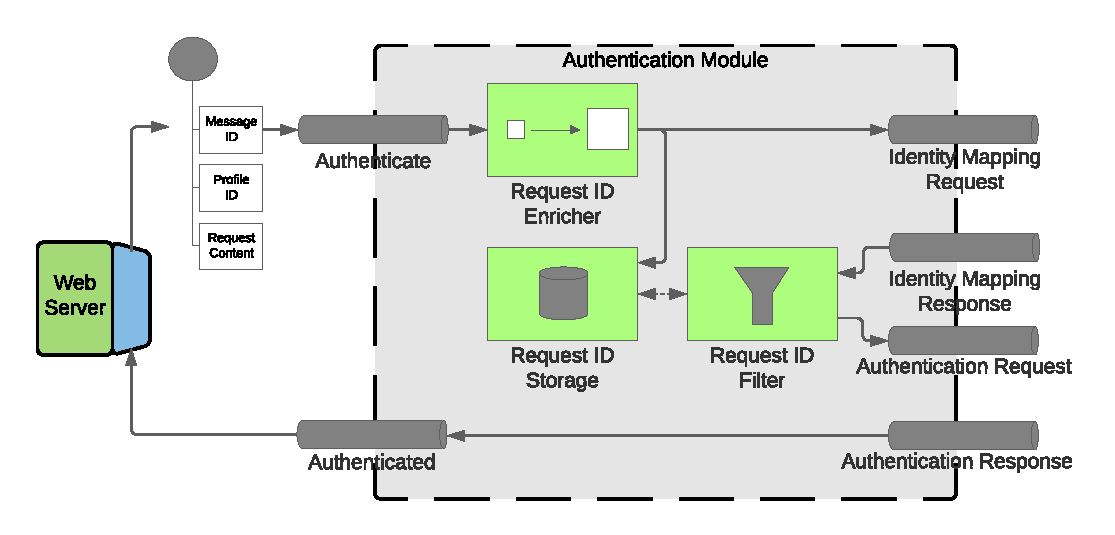
\includegraphics[scale=0.6]{Diagrams/Integration Architecture 1/Technological Integration/15. Authentication.pdf}
\end{center}

When the user visits the web page of the administration portal to apply for an administrative service, he will have to login. To utilize the IMP client for authentication, the web server can use a channel adapter to publish a authentication request concerning a user profile ID and a certain session ID. The adapter publishes a message on the "Authenticate" channel which contains the profile ID and a request content. Next to the session ID, the request content may also include information for presentation to the user like the current time or the IP address of the browser. Similar to previous modules, the relationship ID connected to the profile ID is retrieved and the response published on the "Authentication Request Message, where the "Authentication Message" module further processes the message and sends it to the connector.

Eventually, the IMP client sends a response as message, which the "Authentication Message" module publishes on the "Authentication Response" channel. As the message module already appropriately formatted the response content, the "Authentication" module can simply forward the message to the "Authenticated" channel. The channel adapter of the web server receives the message and based on the session ID contained in the response content can authenticate the browser session.